\documentclass[11pt]{article}

\usepackage{ctex}
\usepackage{amsmath, amssymb}
\usepackage{graphicx}
\usepackage{booktabs}
\usepackage{geometry}
\usepackage{float}
\usepackage{bm}

\geometry{a4paper, margin=2.5cm}
\graphicspath{{figures/}}

\begin{document}

\section{自编码器与自监督学习}

本题在 CIFAR-10 上比较自编码器（AE）、旋转角度预测和掩码自编码器（MAE）三种表示学习
方法。为满足“编码器架构、参数量、输出表示维度尽量一致”的要求，三者共用同一个小型
ViT 编码器，仅在自监督目标和（解码器 / 分类头等）任务相关部件上不同。三个模型均在
CIFAR-10 训练集（$50000$ 张）上预训练，预训练阶段不使用任何类别标签。

\subsection{统一的编码器设计}

把 $32\times32$ 图像切成 $4\times4$ 的块，共 $8\times8=64$ 个块，每块展平为 $48$ 维向量。
编码器为 ViT：线性嵌入到 $192$ 维，加可学习位置编码，经 $6$ 层、$3$ 头的 pre-norm
Transformer，输出 $64$ 个 token 的表示。下游统一表示取这些 token 的均值池化，得到
$\bm{z}\in\mathbb{R}^{192}$。三种方法共享该结构，编码器参数量均为 $2{,}691{,}264$，
表示维度均为 $192$，保证比较公平。

实现上，位置编码先加在全部 $64$ 个位置上、再按可见块的索引 \texttt{gather}，因此编码器
天然支持\textbf{变长输入}：既能编码全部 $64$ 个块（AE、旋转预测、线性探针），也能只编码
MAE 遮蔽后剩下的 $16$ 个块。这正是 MAE 要求的“同一编码器支持遮蔽 $75\%$ 与不遮蔽两种
输入”。三个模型都用 AdamW + 余弦退火、批大小 $128$ 训练，图像按通道做标准化，下文重构误差
均在标准化空间度量。

\subsection{自编码器}

编码器编码全部 $64$ 个块，接一个轻量 ViT 解码器（$2$ 层、$128$ 维），把 $64$ 个 token
映射回 $64\times48$ 的块并拼回整图，以全图重构 MSE 为损失，训练 $50$ 个 epoch。

测试集重构 MSE 为 $\mathbf{9.2\times10^{-5}}$，重构图（图~\ref{fig:ae}）与原图几乎无法区分。
原因是该自编码器没有信息瓶颈：$64$ 个 $192$ 维 token 的中间表示远大于输入的
$64\times48$，编码器只需近似“复制”输入即可让重构误差趋近于 $0$。这一点为第 4 问埋下伏笔
——重构得好并不等于学到了对分类有用的语义表示。

\begin{figure}[H]
    \centering
    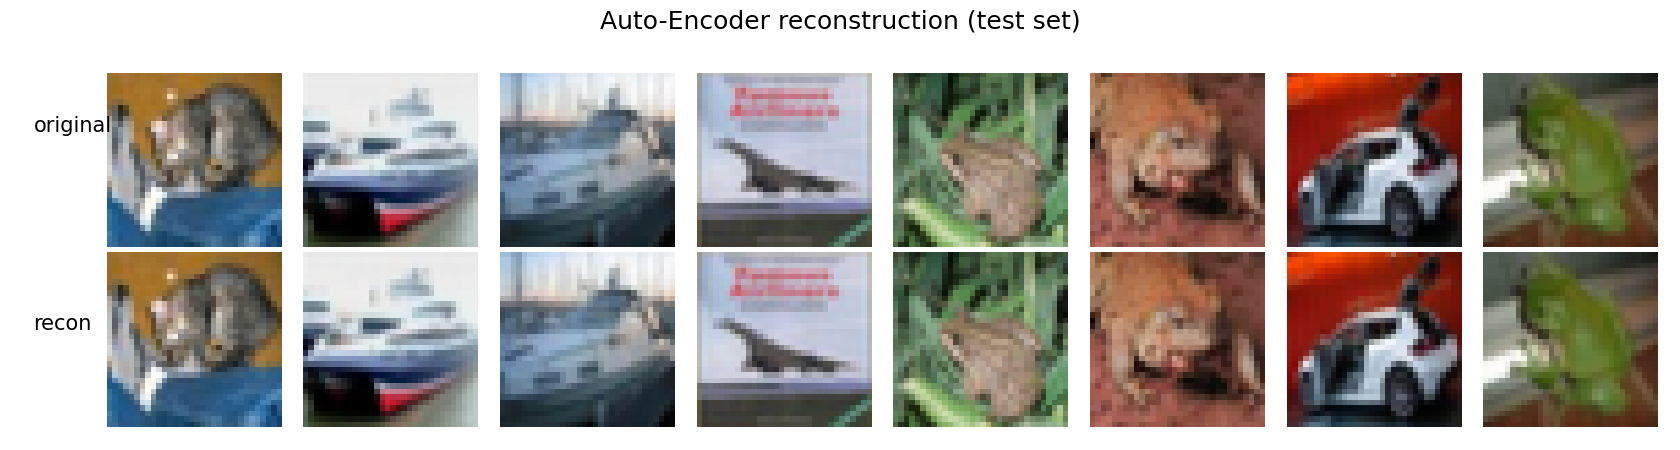
\includegraphics[width=0.85\textwidth]{ae_reconstruction.png}
    \caption{自编码器在测试集上的重构：上排为原图，下排为重构图。}
    \label{fig:ae}
\end{figure}

\subsection{旋转角度预测}

训练时对每张图随机旋转 $0^\circ,90^\circ,180^\circ,270^\circ$（对应标签 $0,1,2,3$），
编码器输出均值池化后接一个线性四分类头，用交叉熵训练模型预测旋转角度，训练 $40$ 个 epoch。
测试时对每张测试图的全部 $4$ 个旋转分别预测并统计总体准确率。

测试集旋转预测准确率为 $\mathbf{56.1\%}$（随机基线 $25\%$）。要判断一张自然图被旋转了多少，
模型必须捕捉“天在上、地在下、物体朝向”等带语义的方向性线索，因此学到的表示比 AE 更偏语义；
但 CIFAR-10 中不少类别（如鸟、猫的局部纹理）方向线索弱，加之小模型容量有限，准确率并不高。

\subsection{掩码自编码器（MAE）}

把 $64$ 个块随机打乱后保留前 $25\%$（即遮蔽 $75\%$，每个 epoch 重新随机），编码器\textbf{只
编码这 $16$ 个可见块}；解码器端按原始顺序用共享的 mask token 补齐到 $64$ 个位置、加解码器
位置编码后经 $2$ 层 ViT 预测所有块，损失只在被遮蔽块上计算 MSE，训练 $80$ 个 epoch。

测试时对每张图固定随机遮蔽 $75\%$，测试样本集上被遮蔽块的重构 MSE 为 $\mathbf{0.265}$。
注意这与 AE 的 $9.2\times10^{-5}$ 不可直接比较：MAE 必须\emph{从看不见的区域猜测}像素，是
远难于 AE“复制可见输入”的任务，正是这个高难度的代理任务迫使编码器学习图像的全局结构与语义。
图~\ref{fig:mae} 给出原图、遮蔽图与重构图：尽管 $75\%$ 的块被遮蔽，模型仍能恢复出物体的
大致轮廓与配色，重构图偏模糊（MSE 损失对不确定区域取均值的固有结果）。

\begin{figure}[H]
    \centering
    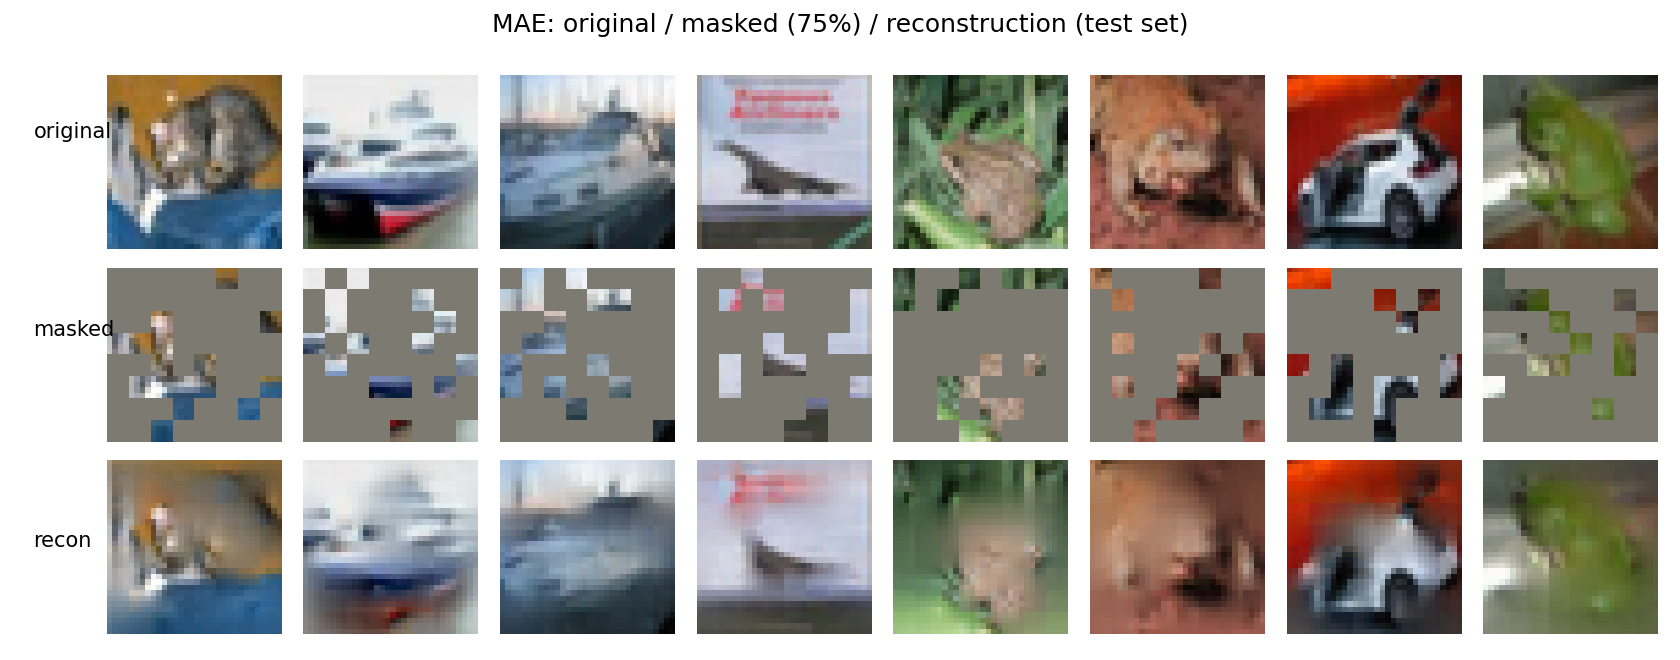
\includegraphics[width=0.85\textwidth]{mae_reconstruction.png}
    \caption{MAE 在测试集上的结果：上排原图，中排遮蔽 $75\%$ 后的输入，下排重构
    （可见块用原图、被遮蔽块用预测填充）。}
    \label{fig:mae}
\end{figure}

\subsection{线性分类评估与表示分析}

冻结上述三个预训练编码器，以其均值池化输出（$192$ 维）为输入，在训练集上用交叉熵训练
线性分类器（此阶段才使用标签），在测试集上比较分类准确率，结果见表~\ref{tab:probe}。

\begin{table}[H]
    \centering
    \caption{三种表示学习方法在 CIFAR-10 测试集上的线性分类准确率（编码器冻结）}
    \label{tab:probe}
    \begin{tabular}{lccc}
        \toprule
         & 自编码器 (AE) & 旋转预测 & MAE \\
        \midrule
        自监督目标（测试集） & 重构 MSE $9.2\times10^{-5}$ & 旋转准确率 $56.1\%$ & 遮蔽块 MSE $0.265$ \\
        线性分类准确率       & $35.4\%$ & $38.8\%$ & $\mathbf{64.1\%}$ \\
        \bottomrule
    \end{tabular}
\end{table}

三种方法的线性分类准确率为 MAE ($64.1\%$) $>$ 旋转预测 ($38.8\%$) $>$ AE ($35.4\%$)。
图~\ref{fig:tsne} 用 t-SNE 把测试集表示降到二维（按真实类别着色），与上述准确率高度一致：

\begin{figure}[H]
    \centering
    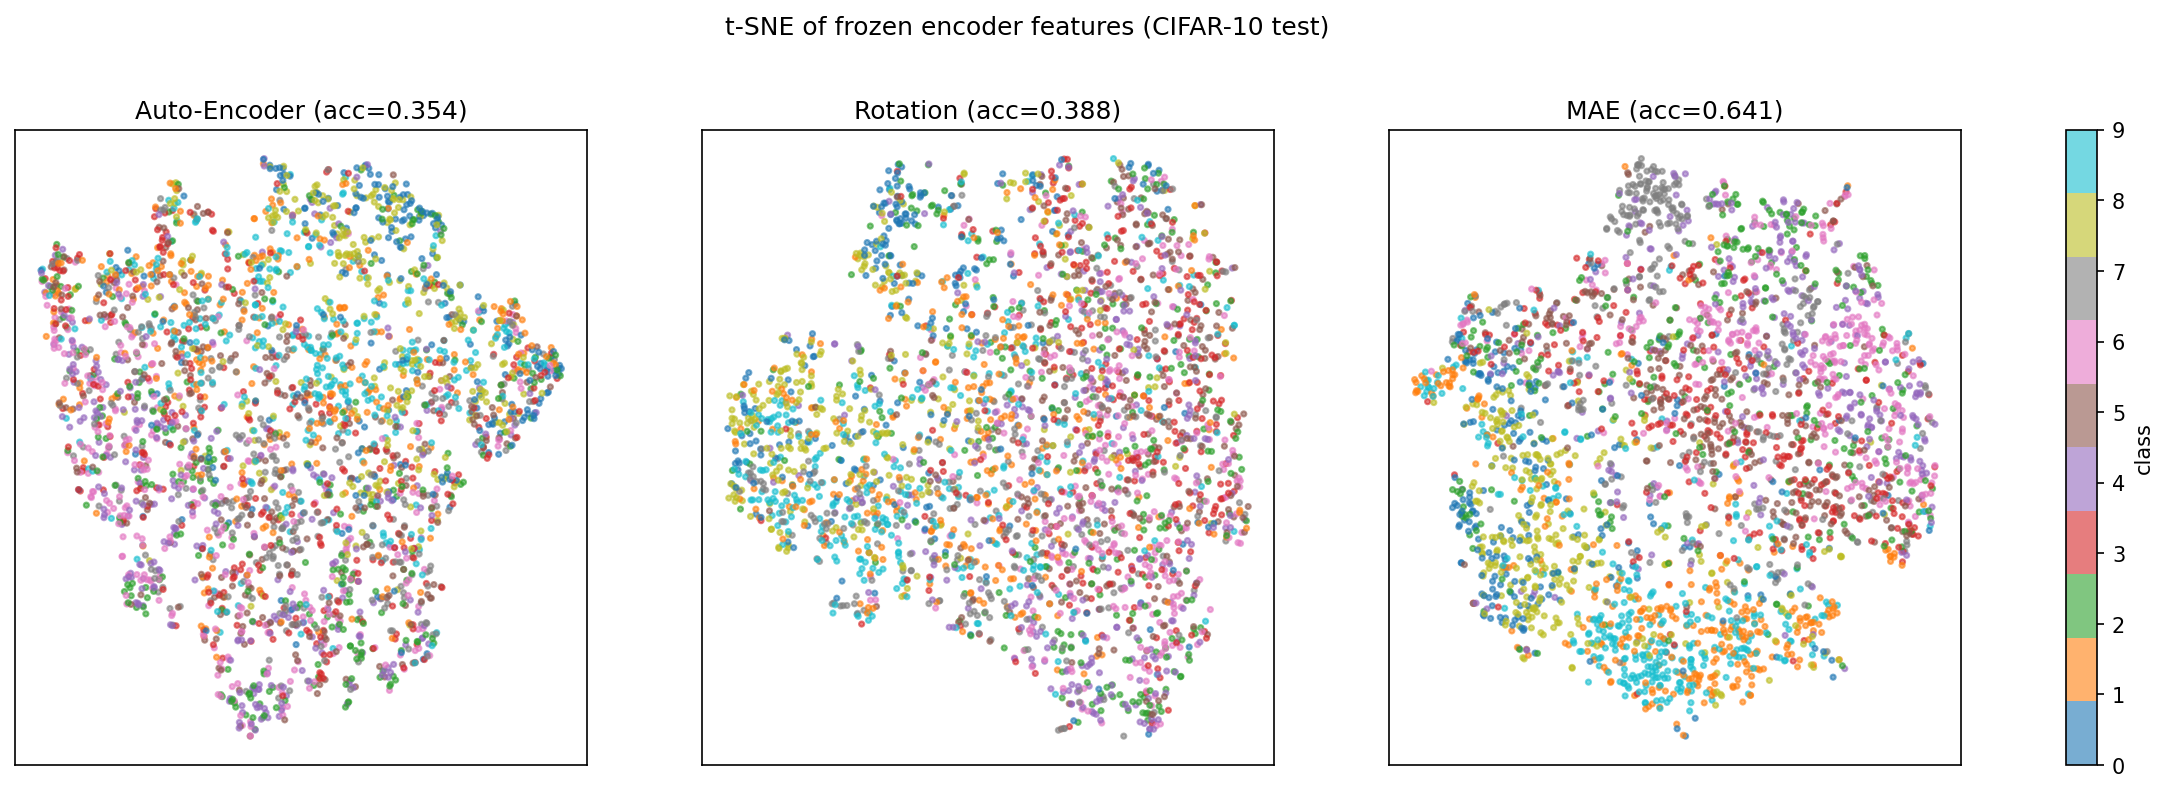
\includegraphics[width=\textwidth]{tsne_features.png}
    \caption{三种冻结编码器在 CIFAR-10 测试集表示上的 t-SNE 可视化（按真实类别着色），
    括号内为对应的线性分类准确率。}
    \label{fig:tsne}
\end{figure}

\paragraph{三种表示有何不同。}
\textbf{AE} 的特征在 t-SNE 中各类高度混杂、几乎没有按类聚集的结构。因为像素级重构损失只
要求“能还原输入”，在没有信息瓶颈时模型倾向于保留低层像素/颜色信息而非语义，重构误差
最低（$9.2\times10^{-5}$）反而对应最差的分类表示——重构质量与语义质量并不一致。
\textbf{旋转预测}的特征出现了一定的成片结构，分类准确率略高于 AE：判别旋转角度需要一些
方向性的语义线索，但这些线索与“类别”只部分相关，且对方向不敏感的类别帮助有限，因此
聚类松散。\textbf{MAE} 的特征在 t-SNE 中呈现最清晰的按类分簇、类间间隔最明显。从可见
$25\%$ 的块去重建被遮蔽区域，要求编码器理解物体的形状、部件关系与上下文等全局语义，这种
高层语义恰好对分类最有用。

\paragraph{哪种方法对分类更有帮助。}
MAE 明显最有利于下游分类（线性准确率 $64.1\%$，约为 AE、旋转预测的 $1.6\sim1.8$ 倍）。
根本原因在于代理任务的“难度/语义性”：AE 的复制式重构几乎不含语义，旋转预测含部分语义，
而 MAE 的高比例掩码重建迫使模型学习可迁移的全局语义表示。这与“掩码图像建模优于像素重构、
也优于多数早期 pretext 任务”的结论一致。

\end{document}
